\documentclass[../summary.tex]{subfiles}

\begin{document}
	
	\section{Demography}
	
	\subsection{Study guide}
	
	Module 3 (Demography) sketches basic insights into the origins and dynamics of population growth. Make sure to understand:
	\begin{itemize}
		\setlength{\itemsep}{0pt}
		\item The link between the industrial revolution and evolutions in mortality
		\item The drivers behind the evolution of fertility rates
		\item The link between evolutions of mortality and fertility
		\item How evolutions of mortality and fertility influence both the demographics and the economic
		growth expectations of societies
	\end{itemize}
	Don’t learn the specific examples by heart; focus on understanding the reasons behind the evolutions.
	
	\subsection{Link between industrial revolution and evolution in mortality}
	The spread of the \textbf{industrial revolution} was \textbf{paired with} a \textbf{decline in mortality}. The reason behind this is that the industrial revolution led to a completely different societal development. 
	\\
	\\
	Before the industrial revolution, most people would produce their goods locally at home and they taught their kids their trades. This changed in the industrial society. People moved to the city and capital became a much more important production factor as production became concentrated and factories had to be built. The people with capital, they need new knowledge, new insights to make their factories more efficient, to make new products, and therefore, they need science and technology. This science and technology will not only be used to make their factories more efficient, but it will also be used to reduce mortality, to have better food, to have new food storage techniques, etc. 
	\\
	\\
	So, this evolution resulted in a totally different society that was developing rapidly and the combination of increased knowledge (a deeper understanding of technology, production methods, and various industrial processes), increased understanding (a better grasp of health issues, living conditions) and a different societal organization (shift from a rural society to cities) also led to a dramatic reduction of mortality rates. 
	
	\subsection{Drivers behind the evolution of fertility rates}
	
	There are a lot of drivers behind the evolution of fertility rates.
	
	\begin{itemize}
		\item \textbf{Reduced Child Mortality:} With improvements in healthcare, sanitation, and overall living conditions, child mortality rates drastically decreased. Parents no longer needed to have a large number of children to ensure that some would survive to adulthood.
		\item \textbf{Social Welfare Systems:} The emergence of social welfare systems, including healthcare and pensions, meant that elderly individuals were no longer solely dependent on their children for support. This reduced the need for large families to ensure care in old age.
		\item \textbf{Educational Investments:} Industrial societies placed a higher value on education. Parents began investing more time and resources in the education of their children, aiming for quality rather than quantity.
		\item \textbf{Wealth of a country}: Wealthier societies have less children
		\item \textbf{Marriage age}: In societies where women marry later, they have less children.
		\item \textbf{Changing parental priorities}: Parents, particularly those with careers and personal aspirations, prioritize investing in their own development. As a consequence, they tend to have fewer children, as raising children requires significant time and financial investments.
		\item \textbf{Education of women}: If women are educated, they are better capable of applying of using contraception correctly. If you use contraception correctly, then you will end up probably with less children. It is also true that if you offer education to women, then of course they need to invest time in that and very few people have children while they study. Also, after their studies, these women very often want to have a job and pursue a career. Because of that, they will have less time to care for children and if there is less time available, that will also lead to having less children. The desire to provide their children with equal or better opportunities than they had further accelerates the decline in the number of children.
	\end{itemize}
	
	\subsection{Link between evolutions of mortality and fertility}
	In general the decline of fertility starts decades after the decline of mortality. Society has to adjust to a higher life expectation before this higher life expectation translates into a lower number of children being born. The only exception to this rule is France in the end of the 18th century where mortality and fertility started to decline at the same time. Scientist suggest that there is a link with the French Revolution. 
	\\
	\\
	The delay between child mortality decline and fertility decline leads to a population increase . The increase of population is higher in developing countries because the knowledge to reduce mortality  was already much more developed by then. This can be seen in figure \ref{fig:fertility-and-mortality-decline}.
	
	\begin{figure}[H]
		\centering
		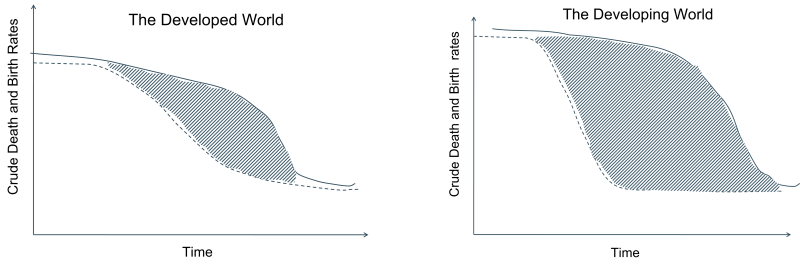
\includegraphics[width=0.7\linewidth]{../images/3-fertility-and-mortality-decline.png}
		\caption{Fertility and mortality decline in the develop(ed)(ing) world}
		\label{fig:fertility-and-mortality-decline}
	\end{figure}
	
	
	\subsection{Influence of mortality and fertility evolution on the demographic and economic growth expectations of societies}
	When there is a decline in mortality, followed by a decline in fertility, there will first be a phase where there are a lot of young people and fewer older people. This is an important phase in the economic development of a society because there are a lot of people wo can produce and contribute to economic growth, while they do not need to take care of a lot of older people. This can result in an economic growth of 7 to 10\% per year during several decades. This growth does however require the right conditions for economic development, with education as its key factor.
	\\
	\\
	This growth will however come to an end. When the mortality and fertility keep declining, there will be a moment when there are a lot of older people with less youngsters. Hence, there will be less people to contribute and more people to take care of. These mature societies will keep growing, but at a much slower pace then before, maybe 1 to 3\% per years. There could be even years where there is no economic growth.
	
\end{document}